\section{Problem Description}
We start off with a sequential program that detects collisions for a particular polygon mesh that is the input of the program. This program is meant to run on a CPU, and we are going to transform part of this program to a parallel program that can be run on a GPU. We will first elaborate on the structure of the program, and after that on the pseudocode for the part of the sequential program we are going to transform.

The program uses 2 complex datastructures: a BHV and an object called Collisions. In the BHV the data of the mesh (vertices, edges and faces), how they are related (which vertices and edges belong to a face), and a binary tree of bounding boxes, which we described in section 1. In the Collisions object, the output is stored, thus the pairs of faces that potentially collide, and eventually the pairs of vertex-face and edge-edge which potentially collide.

The goal of the program is to detect which faces potentially collide, without doing the actual geometric calculations. Using the bounding boxes in the BHV, we try to prune the amount of elements we have to do the geometric calculations on. The first part of the program finds all pairs of faces that might collide, and the second part processes these face-face pairs, and checks whether the collision is a collision of a vertex onto a face, or two edges colliding. The collisions are detected using a displacement vector: a displacement the model undergoes, which leads to collisions in the model. Figure \ref{fig:process} shows the steps of the process, along side the input and output of the process' elements.

\begin{figure}
	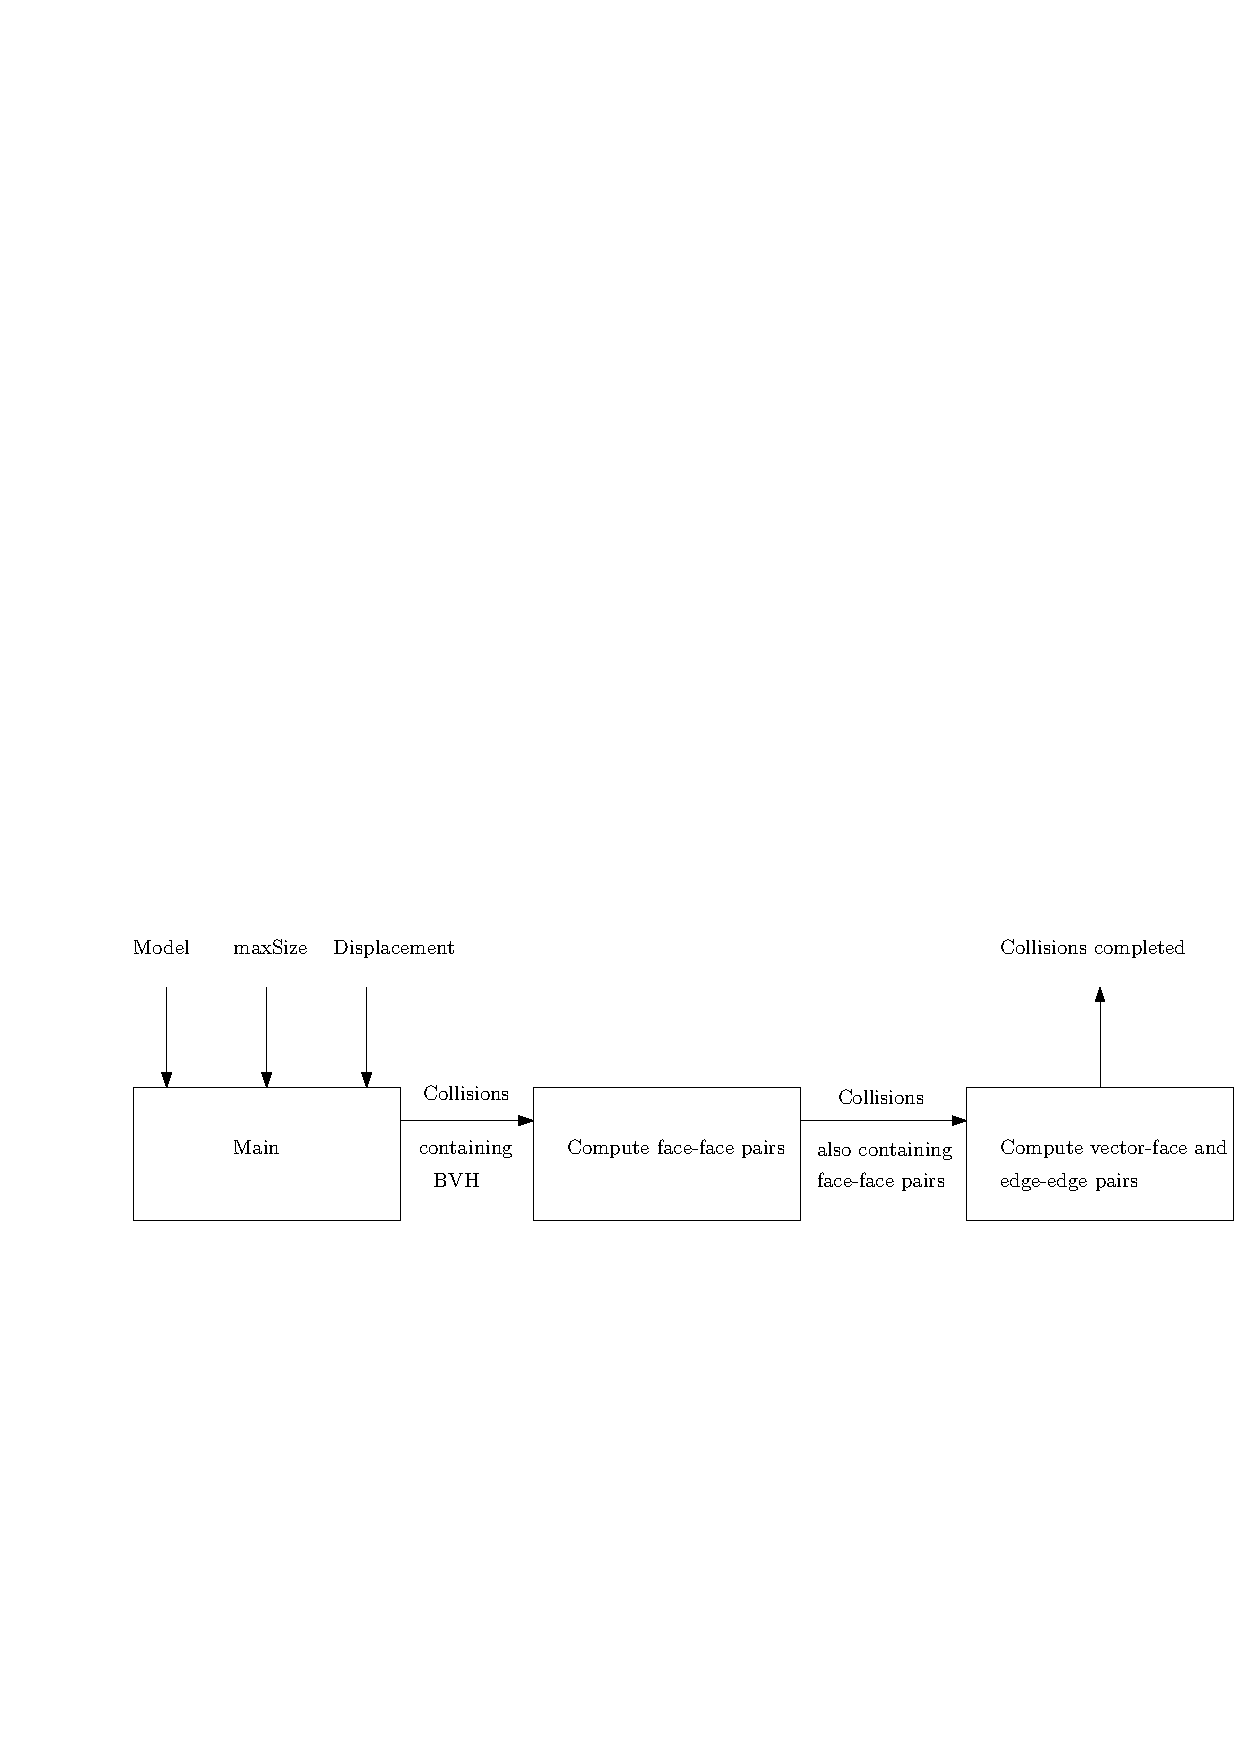
\includegraphics[width=\textwidth]{process.pdf}
	\caption{All steps in the process of finding potential collisions}
	\label{fig:process}
\end{figure}

The procedure that we are going the look into is called \texttt{breakDown}. It is part of the Collisions object and it does the second part of the calculations. This means that the potential face-face pairs are already calculated/available and we want to calculate vertex-face and edge-edge pairs accordingly. The procedure takes a BHV and a vector (the displacement) as input. Algorithm \ref{alg:breakseq} shows the pseudocode for the procedure.

\begin{algorithm}
\caption{breakDown (sequential)}\label{alg:breakseq}
\begin{algorithmic}[1]
\Procedure{breakDown}{$bhv,vector$}
    \For{$faceA\gets 0, \#faces$}
        \ForAll{$i \gets pairs(faceA)$}
            \State $faceB \gets faceIndex(faceA, i)$ \Comment{for each pair with faceA, find index of other face}
            \State $vertices \gets getVertices(faceA)$
            \State $edgesA \gets getEdges(faceA)$
            \State $edgesB \gets getEdges(faceB)$
            \For{$vertex \gets 0, 3$}
                \State $checkVertexFaceCollision(vertices[vertex], faceB)$
            \EndFor
            \For{$edgeA \gets 0, 3$}
                \For{$edgeB \gets 0, 3$}
                    \If{$edgesA[edgeA] < edgesB[edgeB]$} \Comment{avoid doubles}
                        \State $checkEdgeEdgeCollision(edgesA[edgeA], edges[edgeB])$
                    \EndIf
                \EndFor
            \EndFor
        \EndFor
    \EndFor
\EndProcedure
\end{algorithmic}
\end{algorithm}

The \texttt{for all} in line 3 has an upperbound \texttt{maxSize}, which is a field of the Collisions object. A small detail for the check-functions in line 9 and 14: they both also store the result in an array with the same upperbound \texttt{maxSize} to the amount of results per vertex/edge. Furthermore, line 13 makes sure that pairs of edge-edge collisions are stored in such a way that for each pair $(X,Y)$ that is stored, it holds that $X < Y$, and $Y <= X$ does not exist.

If we look into the time complexity of this procedure, we get $\#faces *  maxSize$ times the calculations within the loops. The get-functions all have constant time complexity, since they are plain array inspections. The check-functions are also constant time, as they are checking bounding box bounds against each other and storing the value in an array. This means that we get $3$ (vertices) and $3*3$ (edges times edges) times a constant calculation. This leaves us with a time complexity of $O(\#faces *  maxSize)$.

We want to improve on this running time bound by adjusting the procedure in such a way that it can leverage parallellism on a GPU.
